\documentclass{ximera}
\typeout{Start loading xmPreamble.tex}%

% Extra macros loaded automatically by all documents of class 'ximera' or 'xourse'

\newcommand{\PP}{\mathbb{P}}
\newcommand{\EE}{\mathbb{E}}
\newcommand{\Var}{\mathrm{Var}}
\newcommand{\indep}[2]{\PP\left(#1 \cap #2\right) = \PP\left(#1\right) \cdot \PP\left(#2\right)}
\newcommand{\cond}[2]{\frac{\PP( #1 \cap #2)}{\PP(#2)}}
\newcommand{\pdf}{\text{probability distribution function}}

% Ximera already defines theorem-like environments:
% theorem, lemma, corollary, example, definition, etc.
% So do NOT redefine them here.

\usepackage{tikz}
\usetikzlibrary{positioning, arrows.meta}

\usepackage{multicol}
\usepackage{enumitem}
\usepackage{caption}
\usepackage{amsmath,amssymb,amsfonts}
\usepackage{mathtools}
\usepackage{graphics}
\usepackage[T1]{fontenc}
\usepackage{colortbl}
% \usepackage{fouriernc}
\usepackage{marvosym}
\usepackage{color}

\providecommand{\Lightning}{\ensuremath{\text{\sffamily\bfseries !}}}

\def\arrvline{\hfil\kern\arraycolsep\vline\kern-\arraycolsep\hfilneg}

\title{Chapter 1}
\begin{document}
\begin{abstract}
\end{abstract}
\maketitle
\section{Chapter 1}

\subsection{Basic Examples and Definitions}\label{Beg}
We begin our class with some basic examples of probability.

\begin{enumerate}
\item

Roll a \underline{fair} six--sided dice. The set of possible outcomes is
$$
\{1,2,3,4,5,6\}.
$$
The probability of each outcome is $1/6$.

\item
Flip a \underline{fair} coin. The set of possible outcomes is
$$
\{H,T\}.
$$
(Note that outcomes don't have to be numbers). The probability of each outcome is $1/2$.

\item
Roll a \underline{fair} fix--sided dice and independently flip a \underline{fair} coin: What is the set of possible outcomes and what is the probability of each outcome?

\end{enumerate}

More generally, we have the definition:

\begin{definition}
The set of all possible outcomes is called the \textit{sample space}, and is usually denoted by $\Omega$ (this is the capital Greek letter omega). Outcomes are required to be mutually exclusive. 
\end{definition}

Even in the above examples, we can ask more interesting questions. For example, if we roll a six--sided die, what is the probability of obtaining an even number?

\Lightning \Lightning \      From the class discussion, we saw (I hope) two ways to answer the question, which I personally call ``the addition/summation method'' and ``the symmetry method.'' (Nobody else calls it this, but I find it a helpful way of thinking). This problem was simple enough that both methods are equally good, but for more difficult problem, we'll find that only one method works. As you progress through the class, please keep in mind that there are often multiple ways to approach a problem, but sometimes one will be much better than the others, or only one will work.  \Lightning \Lightning

For the previous question, we had to use something more general than an outcome, which we call an event:

\begin{definition}
An \textit{event} is a collection of outcomes; in other words, it is a subset $E\subseteq \Omega$. Note that an event can be a single outcomes, the empty set, or all of $\Omega$.
\end{definition}
Personally, I find the language a little strange that an empty set is still an event. It would be like if a stamp collector sold all of her stamps, then she's still a stamp collector, it's just that her collection is empty.

We will actually consider probabilities of events, not of outcomes. This helps us broaden the range of interesting questions we can ask.

\begin{definition}
A \textit{probability law} $\PP$ assigns a probability to all events $E\subseteq \Omega$. This is denoted $\PP(E)$. 
\end{definition}

In the previous example, we have
$$
\PP(\{2,4,6\}) = 1/2 \text{ or } \PP(\text{even number})=1/2.
$$
(It's ok the describe the event in words.)

\Lightning \Lightning \ I was once reading the book ``Russian for the Mathematician,'' and the author begins with the pronunciation of the Cyrillic letters. He explained that most readers subconsciously sound the words out loud without realizing it, and not knowing pronunciation makes it harder to read. I won't use any Russian in this class, of course, but math is its own language with its own pronunciation. For example, $f(x)$ is pronounced ``f of x'' because

\begin{center}
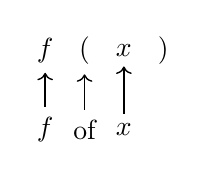
\begin{tikzpicture}
\node at (0,0) (aa)  {$f$};
\node at (0.5,0) (bb) {$($};
\node at (1,0) (cc)  {$x$};
\node at (1.5,0)  {$)$};
\node at (0,-1) (a) {$f$};
\node at (0.5,-1) (b) {of};
\node at (1,-1) (c) {$x$};
\draw (aa) edge[out=-90,in=90,<-, line width=0.5pt] (a);
\draw (bb) edge[out=-90,in=90,<-, line width=0.5pt] (b);
\draw (cc) edge[out=-90,in=90,<-, line width=0.5pt] (c);
\end{tikzpicture}
\end{center}
So similarly, $\PP(E)$ is pronounced ``probability of event''
\begin{center}
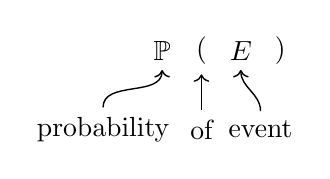
\begin{tikzpicture}
\node at (0,0) (aa)  {$\PP$};
\node at (0.5,0) (bb) {$($};
\node at (1,0) (cc)  {$E$};
\node at (1.5,0)  {$)$};
\node at (-0.75,-1) (a) {probability};
\node at (0.5,-1) (b) {of};
\node at (1.25,-1) (c) {event};
\draw (aa) edge[out=-90,in=90,<-, line width=0.5pt] (a);
\draw (bb) edge[out=-90,in=90,<-, line width=0.5pt] (b);
\draw (cc) edge[out=-90,in=90,<-, line width=0.5pt] (c);
\end{tikzpicture}
\end{center}
Probability is much more ``applied'' than other math courses: a lot of doing probability is understanding how to translate back and forth between math language and plain language.  \Lightning \Lightning 

\subsection{Kolmogorov's Axioms}
We need to make certain assumptions, also known as axioms, about $\mathbb{P}$ . These are called Kolmogorov's\footnote{I like giving historical information about anyone whose name I reference. Some trivia about Kolmogorov is that he did statistical analysis about artillery fire for the Soviet Union during World War II. For example, if it takes 5 hits to destroy a target, how many shots should you fire to ensure a 95 percent probability of destroying the target?} axioms, published in 1933.

\begin{enumerate}
\item ({\color{red} Nonnegativity)}: All events $E\subseteq \Omega$ of nonnegative probability. In symbols, $\mathbb{P}(E) \geq 0$.

\item {\color{red} (Normalization)}: The sample space $\Omega$ has probability $1$. In symbols, $\mathbb{P}(\Omega)=1$.

\item {\color{red} (Countable additivity)}: If $A_1,A_2,\ldots$ is a finite or countable collection of disjoint (mutually exclusive) events, then
$$
\mathbb{P}(A_1 \cup A_2 \cup \cdots ) = \mathbb{P}(A_1) + \mathbb{P}(A_2) + \ldots
$$
\end{enumerate}

The first two axioms are relatively straightforward, but let's discuss the third one some more. 

{\color{lime} First, a remark on notation}: In math, the symbols $\cup$ and $\cap$ mean union and intersection respectively. (The ``u'' in union looks like the $\cup$). In probability, these will mean ``or'' and ``and.'' In predicate logic, the symbols $\vee$ and $\wedge$ are used for ``or'' and ``and'' (the $\wedge$ looks like the ``A'' in ``And''). I'll stick with $\cup$ and $\cap$, but you can use whatever notation makes more sense to you. Do not, however, use the computer programming notation $|$,$||$, because this will mean something else later.

Second, note that it is necessary to require mutually exclusive events. As a counterexample, let's say we tried to apply additivity to the events $\{2,4\}$ and $\{4,6\}$ in the die roll example. Then $\{2,4\} \cup \{4,6\} = \{2,4,6\}$, and we would conclude that
\begin{align*}
\PP(\{2,4,6\}) &= \PP(\{2,4\}) + \PP(\{4,6\}) \\
&= \quad 1/3 \quad + \quad  1/3\\
&=2/3,
\end{align*}
which is just silly.

At this point, you might be wondering why we (mathematicians) chose these three axioms for probability theory. There are two basic answers: the first is that most other reasonable assumptions can be proved from these three axioms, and the second is that these axioms combine both discrete and continuous probability.

\subsubsection{Using Kolmogorov's axioms for general formulas}
Here's what I mean by proving a result from these three axioms. Think about this statement:
\begin{equation}\label{Ex1}
\text{ if } E_1 \text{ and } E_2 \text{ are two events such that } E_1 \subseteq E_2, \text{ then } \PP(E_1) \leq \PP(E_2).
\end{equation}
This makes sense intuitively: if we add more outcomes to an event, the probability can either increase or stay the same, but it can't decrease. The proof would go like this:
\begin{proof}
Let $E_2-E_1$ denote the set of outcomes in the event $E_2$ that are not in $E_1$. The two events $E_1$ and $E_2-E_1$ are disjoint, and their union is $E_2$. So by additivity,
$$
\PP(E_2) = \PP(E_1 \cup (E_2-E_1)) = \PP(E_1) + \PP(E_2-E_1).
$$
By non--negativity, 
$$
\PP(E_2-E_1) \geq 0.
$$
So therefore $\PP(E_2)\geq \PP(E_1)$. Note that we did not need to use the normalization axiom.
\end{proof}

Here's another example of something that can be proved from Kolmogorov's axioms: for \textit{any} events $E_1,E_2$ (disjoint or not),
$$
\PP(E_1 \cup E_2) = \PP(E_1) + \PP(E_2 ) - \PP(E_1 \cap E_2).
$$
It is not immediately obvious why this is true, but it becomes slightly more clear if you draw a picture:
\begin{center}
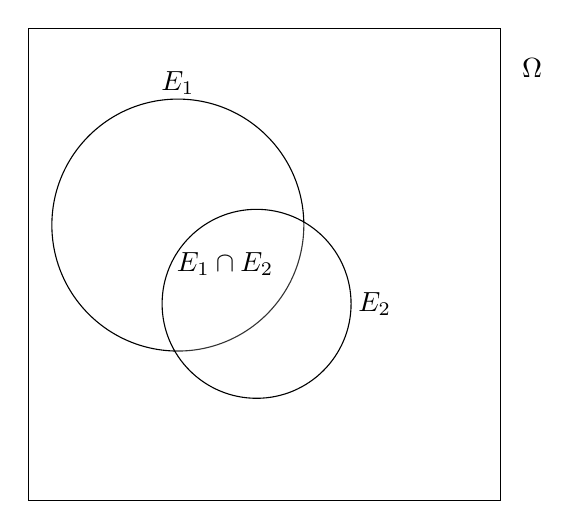
\begin{tikzpicture}
\draw [draw=black] (11.1,5.5) rectangle ++(6,6);
\filldraw [fill=white, fill opacity=0.2, draw=black] (13,9) circle (1.6);
\filldraw [fill=white, fill opacity=0.2, draw=black] (14,8) circle (1.2);
\node at (13,10.8)  {$E_1$};
\node at (15.5,8) {$E_2$};
\node at (13.6,8.5) {$E_1 \cap E_2$};
\node at (17.5,11) {$\Omega$};
\end{tikzpicture}
\end{center}
A good way to start a problem if you're stuck is to draw a picture to help you understand what's going on. This is actually how most mathematicians start problems. As an example, if $E_1 = \{2,4\}$ and $E_2 = \{4,6\}$ (as before), then
\begin{align*}
\PP(\{2,4,6\}) &= \PP(\{2,4\}) + \PP(\{4,6\}) - \PP(\{4\}) \\
&= \quad 1/3 \quad + \quad  1/3  \quad \quad - 1/6\\
&=  1/2,
\end{align*}
which is correct.

\subsubsection{Discrete v. Continuous Probability}
In addition to providing foundations for proving other probability results, Kolmogorov's axioms also unify discrete and continuous probability. Prior to Kolmogorov, discrete and continuous probability were viewed as two separate branches of mathematics. This distinction still exists (to a lesser extent) currently. For example, I was at a large probability conference (300+ participants), and for the introduction to one of the talks, the organizer credited the speaker for convincing him to move from discrete probability to continuous probability. Even the class and textbook is naturally split between discrete probability (the material up to midterm \#1, which covers chapters 1-2 of the textbook) and continuous probability (the material from midterm \#1 to midterm \#2, which covers chapters 3-4 of the textbook), before the limiting theorems in chapter 5, which incorporate both discrete and continuous probability. Let's briefly discuss the contrasts between the discrete and the continuous in probability theory -- hopefully this will give you an overview of the class and where we're going.

In the examples of die--rolling and coin--flipping, there were a finite number of outcomes, each equally likely. We can find the probability of each outcome by taking the inverse of the number of total outcomes.  If the number of total outcomes is infinite, then we need to modify our way of thinking. First, we establish some terminology.

\begin{definition}
A probability law $\PP$ on a sample space $\Omega$ (finite or infinite) is called \textit{uniform} if all the outcomes have the same probability.
\end{definition}

For example, uniforms are uniform because they all look the same. 

No, seriously, as an actual example, let $\Omega$ be the interval $[0,1)$ and let $\PP$ be uniform on $\Omega$. Consider the event $E=[0,1/3)\subset \Omega$. What do you think the value of $\PP(E)$ is? And how would you prove it from Kolmogorov's axioms?

From the class discussion, it looks like most of you think it should equal $1/3$. Here's how to use Kolmogorov's axioms. Define 
$$
p:= \mathbb{P}([0,1/3)).
$$
If we add $1/3$ to the interval $[0,1/3)$, we get $[1/3,2/3)$. If we add $1/3$ again, we get $[2/3,1)$. Because $\mathbb{P}$ is uniform, we must have
$$
p=\PP([0,1/3)) = \PP([1/3,2/3)) = \PP([2/3,1)).
$$
Now, note that $[0,1/3) \cup [1/3,2/3) \cup [2/3,1) = [0,1)=\Omega$, and all three intervals are disjoint. So by the additivity axiom,
$$
\PP(\Omega) = \PP([0,1/3)) + \PP([1/3,2/3)) + \PP([2/3,1)) = 3p.
$$
By normalization,
$$
\PP(\Omega)=1.
$$
So $1=3p$, which means that $p=1/3$.

This approach is what I (personally) called the ``symmetric method'' -- it uses that the three intervals $[0,1/3),[1/3,2/3),[2/3,1)$ are basically just the same interval shifted over, so there's symmetry between them. What if we tried using the ``addition method''? In other words, what if try to find the probability of a single outcome and then try to add them together?

I'll claim that trying to use addition won't work, because the probability of each outcome is $0$, and adding $0$ over and over will only give you $0$. I'll give two ways to see why this is true. Let $p$ be the probability of a single outcome. In symbols,
$$
p = \PP(\{x\}).
$$
Because $\PP$ is uniform, the value of $p$ does not depend on $x$. Since $p$ doesn't depend on $x$, we can take $x=0$. Let $E_n$ denote the event that you picked a number between $0$ and $1/n$; i.e. 
$$
E_n:=[0,1/n)\subseteq \Omega.
$$
Since $0 \in [0,1/n)$, we must have by \eqref{Ex1} that $p\leq \mathbb{P}(E_n)$ for every $n$. But $\PP(E_n)=1/n$ (as we saw before in the case $n=3)$, so $p\leq 1/n$ for every $n$. Since $p\geq 0$  by the non--negativity axiom, then $p$ must satisfy $0\leq p \leq 1/n$ for every $n$. By the sandwich theorem\footnote{Hopefully you're comfortable with limits.} (from Calc I),
$$
0 \leq p \leq \lim_{n\rightarrow \infty} \frac{1}{n} = 0,
$$
so $p=0$.

That was the first way; here is the second way. Let $E_n$ be the event
$$
E_n:= \{1/2,1/3,1/4,1/5,\ldots,1/n\}.
$$
By additivity,
$$
\mathbb{P}(E_n) = \mathbb{P}(\{1/2\}) + \mathbb{P}(\{1/3\}) + \ldots + \mathbb{P}(\{1/n\}).
$$
Since $\PP$ is uniform, this means that $\mathbb{P}(E_n) = pn$. Every probability is between $0$ and $1$, so $0\leq pn \leq 1$ for every $n$. Again, by the sandwich theorem, this means that $p=0$.

So if the addition/summation method doesn't work, what will? It turns out that we replace summation with integration. In this example,
$$
\PP([a,b]) = \int_a^b 1 \cdot dx = b-a.
$$
This is the key difference between discrete and continuous probability -- the former uses sums and the latter uses integrals. Integration is essentially a continuous version of summation. This is even shown in the notation. The summation symbol $\Sigma$ is a the greek capital sigma, which is the analog of the letter S. The integration symbol $\int$ was a long S, before going out of use in the early 1800s. For example, this is the cover of ``Paradise Lost'' by John Milton:

\begin{center}
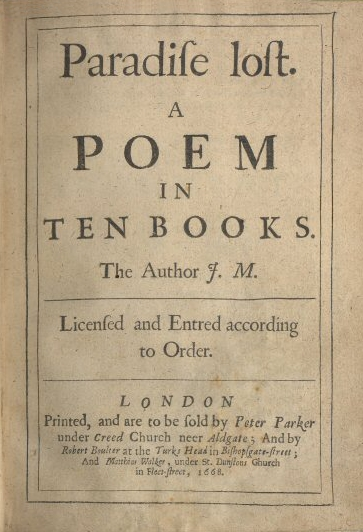
\includegraphics{Milton_paradise.jpg}
\end{center}

\Lightning \Lightning  A lot (and I mean, a \textit{lot}) of the examples, notations and definitions used in probability are based on understanding the distinction between discrete and continuous probability. If you're not clear on the distinction, you'll probably have a rough time preparing for the final, where you'll be expected to know both discrete \textit{and} continuous probability. \Lightning \Lightning


\subsection{Independence}
In the third example of section \ref{Beg}, I used the word ``independent'' to describe the die roll and the coin flip. Most of you ``intuitively'' understood the meaning of the word in the context. However, we need to translate the word ``independent'' from plain language to math language.

So what's the definition of independence mathematically? We start with an example. Suppose we roll two dice, one of which is red and one of which is green; then the state space is 
$$
\Omega = \{1,2,3,4,5,6\} \times  \{1,2,3,4,5,6\} 
$$

We can view $\Omega$ visually as a grid:

\begin{center}
$\Omega$ \quad \quad \quad \quad \quad \quad \quad \text{green} \quad \quad \quad \quad \

\text{red} \quad
\begin{tabular}{ | c | c | c | c | c | c | } 
\hline  11  & 12  & 13 & 14 & 15 &  16  \\ \hline
 21 &  22  & 23 & 24 & 25 & 26  \\ \hline
 31 & 32 & 33  & 34 & 35  & 36  \\ \hline
 41 & 42 & 43 & 44  & 45  & 46 \\ \hline
 51 & 52 & 53 & 54  & 55 &  56 \\ \hline
61 & 62 & 63 &  64 & 65 & 66  \\ \hline
\end{tabular}
\end{center}
If both die are fair and the rolls are independent, then the probability law $\PP$ is uniform. So let's ask the following questions:

(a) What is the probability that the red dice shows a $2$ or a $3$?

(b) What is the probability that the green dice shows a $5$?

(c) What is the probability that both (a) \textit{and} (b) occur?

Questions (a) and (b) can be answered (relatively) straightfowardly. Because the two dice are independent of each other, they ``don't care'' about the other die, so to say. To answer (a), we can pretend the green die doesn't exist; likewise to answer (b), we can pretend the red die doesn't exist. So we get the answers $1/3$ and $1/6$, respectively.

To approach (c), we can start by coloring in the grid (pretend that brown = green + red):

\begin{center}
$\Omega$ \quad \quad \quad \quad \quad \quad \quad \text{green} \quad \quad \quad \quad \

\text{red} \quad
\newcolumntype{g}{>{\columncolor{green}}c}
\begin{tabular}{ | c | c | c | c | g | c | } 
\hline  11  & 12  & 13 & 14 & 15 &  16  \\ \arrayrulecolor{red}\hline
\rowcolor{red} 21 &  22  & 23 & 24 & \cellcolor{brown} 25 & 26  \\  \hline
\rowcolor{red} 31 & 32 & 33  & 34 & \cellcolor{brown} 35  & 36  \\ \hline \arrayrulecolor{black}
 41 & 42 & 43 & 44  & 45  & 46 \\ \hline
 51 & 52 & 53 & 54  & 55 &  56 \\ \hline
61 & 62 & 63 &  64 & 65 & 66  \\ \hline
\end{tabular}
\end{center}
We can count two boxes out of thirty--six, to get $2/36=1/18$ as the answer. Another approach is to view $\Omega$ as a square of width and height $1$.  (By the normalization axiom, the area of $\Omega$ should be $1$). Then the red box is a rectangle of height $1/3$ (the answer to (a)) and width $1$, and the green box is a rectangle of width $1/6$ (the answer to (b)) and height $1$. Then the brown rectangle has height $1/3$ and width $1/6$, so its area is $1/3\cdot 1/6=1/18$.

From this example, it is reasonable to make the definition:

\begin{definition}
Two events $E_1$ and $E_2$ are \textit{independent} if
$$
\PP(E_1 \cap E_2) = \PP(E_1) \cdot \PP(E_2).
$$
\end{definition}

\Lightning \Lightning\ \  It is very easy to neglect the normalization axiom, because it is so ``obvious.'' But if you viewed the red box as having area $12$ and the green box as having area $6$, then you would find that $12\cdot 6$ equals $2$ ... which it doesn't. \Lightning \Lightning

The concept of independence can be tricky to grasp. Here are some questions to get you thinking:

Suppose that the events $E_1$ and $E_2$ are disjoint. Are $E_1$ and $E_2$ independent?
\begin{center}
\begin{tikzpicture}
\draw [draw=black] (11.1,5.5) rectangle ++(6,6);
\filldraw [fill=white, fill opacity=0.2, draw=black] (13,9) circle (1.6);
\filldraw [fill=white, fill opacity=0.2, draw=black] (16,8) circle (0.8);
\node at (13,10.8)  {$E_1$};
\node at (15.5,7) {$E_2$};
\node at (17.5,11) {$\Omega$};
\end{tikzpicture}
\end{center}
If you found this question confusing -- don't worry, it's a common mistake (even one mentioned in the book). Part of the confusion is due to the word ``independent.'' We expect independent events to ``not care'' about each other, which is better described as ``indifference.'' The example that I like is that when the United States declared ``independence'' from Great Britain, it didn't mean that the US didn't care about Great Britain -- to the contrary, the US probably cared a great deal. So ``indifference'' is probably the better term -- but unfortunately, the term ``independent'' already stuck.

Another tricky question: what if the two events $E_1$ and $E_2$ satisfy $\PP(E_1 \cap E_2) = \PP(E_1) \cdot \PP(E_2)$, but the two sides of the equation are just ``accidentally'' equal? (Meaning that they're not viewed as rectangles). They're still independent (from a mathematical definition), even if it feels like they shouldn't be. This is just because the ``English--to--math'' translation is imperfect. (It's possible to modify the Kolmogorov axioms to address this, but then the axioms become more complicated).

Here's a more concrete question, courtesy of the weather app on my phone. Let $E_1$ be the event that it will rain between 1--2pm, and let $E_2$ be the event that it will rain between 2--3pm. My phone says that both $E_1$ and $E_2$ have probability 90\% percent of occurring. Are $E_1$ and $E_2$ independent?


We also need to define independence for $n$ events $E_1,\ldots,E_n$. In this case, there are two definitions.

\begin{definition}
We say that the events $E_1,\ldots,E_n$ are \textit{pairwise independent} if 
$$
\PP(E_i \cap E_j) = \PP(E_i) \cdot \PP(E_j)
$$
for every $1\leq i < j \leq n$.

The events $E_1,\ldots,E_n$ are \textit{mutually independent} if 
$$
\PP\left(\bigcap_{i \in S} E_i\right) = \prod_{i \in S} \PP(E_i)
$$
for every subset $S\subseteq \{1,\ldots,n\}$.
\end{definition}

The notation for mutual independence can be confusing, so here's an example. The three events $E_1,E_2,E_3$ are mutually independent if
\begin{align*}
&\indep{E_1}{E_2} \\
&\indep{E_1}{E_3}\\
&\indep{E_2}{E_3}\\
\mathbb{P}(E_1&\cap E_2  \cap E_3) = \PP(E_1) \cdot \PP(E_2) \cdot \PP(E_3).
\end{align*}

Note that $\mathbb{P}(E_1\cap E_2  \cap E_3) = \PP(E_1) \cdot \PP(E_2) \cdot \PP(E_3)$ is \textit{not} enough to guarantee mutual independence. 

\newpage



\newpage


\subsection{Conditional Probability}
The concept of independent events is a little bit odd under Kolmogorov's axioms. In contrast, conditional probability is a lot nicer, and this is the topic here.

The idea of conditional probability is that your probability law $\PP$ should change when you're given new information. For example, your estimated probability that somebody has a cold should change if you hear them cough. This would be denoted
$$
\PP(\text{cold}) \text{ and } \PP(\text{cold} | \text{cough}).
$$

{\color{lime} If you've taken a statistics class}, you might have seen $H$ represent a hypothesis and $E$ represent evidence, and $\PP(H)$ represent the prior probability, $\PP(H\vert E)$ represent the posterior probability, and $\PP(E \vert H)$ represent the likelihood. This is the same idea that we're discussing here. 

The math--to--English translation for $\PP(E \vert E')$ looks like this:
\begin{center}
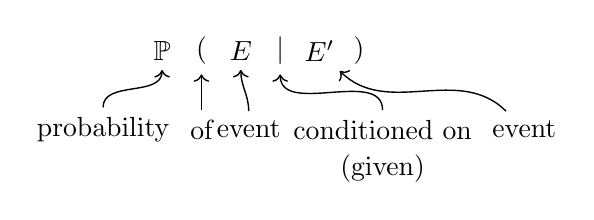
\begin{tikzpicture}
\node at (0,0) (aa)  {$\PP$};
\node at (0.5,0) (bb) {$($};
\node at (1,0) (cc)  {$E$};
\node at (1.5,0) (dd)  {$\vert$};
\node at (2,0) (ee)  {$E'$};
\node at (2.5,0)  {$)$};
\node at (-0.75,-1) (a) {probability};
\node at (0.5,-1) (b) {of};
\node at (1.1,-1) (c) {event};
\node at (2.8,-1) (d) {conditioned on};
\node at (2.8,-1.5) {(given)};
\node at (4.6,-1) (e) {event};
\draw (aa) edge[out=-90,in=90,<-, line width=0.5pt] (a);
\draw (bb) edge[out=-90,in=90,<-, line width=0.5pt] (b);
\draw (cc) edge[out=-90,in=90,<-, line width=0.5pt] (c);
\draw (dd) edge[out=-90,in=90,<-, line width=0.5pt] (d);
\draw (ee) edge[out=-45,in=135,<-, line width=0.5pt] (e);
\end{tikzpicture}
\end{center}
Sometimes we'll say ``given the event $E$'' rather than ``conditioned on the event $E$''.

So what's the definition of conditional probability, from a mathematical perspective? We start with an example. Someone tells you that after two independent rolls of a fair die, the sum is $5$. What is the probability that the first roll is a $4$?

The first step I like to take is to translate the problem from English to math. Our sample space is
$$
\Omega := \{1,2,3,4,5,6\} \times \{1,2,3,4,5,6\}
$$
and the probability law $\PP$ is the uniform probability law. Let $E'$ be the event that the sum of the two rolls is $5$ and let $E$ be the event that the first roll is $4$. The question is then asking for the value of $\PP(E \vert E')$.

There are two possible approaches here. The first approach is to restrict our sample space to rolls where the sum is $5$, since we're given the information that this has already occurred. In other words, we're excluding outcomes where the sum is not $5$. Then our ``updated'' sample space is just $E'$, which is
$$
E' = \{ (4,1),(3,2),(2,3),(1,4)\}
$$
and the ``updated'' probability law is still uniform. We see that only one of these four outcomes is in the event $E$, so the answer is $1/4$.

The second approach involves counting the outcomes. In order for both events $E$ and $E'$ to occur, we can think of a two-step process. First, $E'$ must occur; second, given the knowledge that $E'$ occurred, then $E$ must occur. So
$$
\PP(E \cap E') = \PP(E') \PP(E \vert E').
$$
In the example here, if the first roll is $4$ and the sum of two rolls is $5$, then the second roll must be a $1$, so $E\cap E' = \{(4,1)\}$. So $\PP(E\cap E')=1/36$. Since $E'$ consists of four outcomes, the probability of $E'$ is given by $\PP(E')=4/36$. Therefore
$$
\PP(E \vert E') = \frac{\PP(E \cap E') }{\PP(E') } = \frac{1/36}{4/36} = \frac{1}{4}.
$$
Notice that these two approaches lead to the same answer. 

From the second approach in this example, it is natural to make the definition, which holds in general:

\begin{definition}
For two events $E$ and $E'$, the probability of $E$ conditioned on $E'$ is
$$
\PP(E \vert E') = \frac{\PP(E \cap E') }{\PP(E') } . 
$$
If $\PP(E')=0$, then $\PP(E \vert E')$ is undefined.
\end{definition}

If the two events $E$ and $E'$ are independent, then we should expect that $\PP(E \vert E')$ equals $\PP(E)$. Intuitively, if you're given the information that event $E'$ has occurred, and $E'$ is completely unrelated to the event $E$, then your probability of $E$ should be unchanged. (For example, the probability that it will rain tomorrow should not change with the knowledge of last night's Cubs score). And indeed, if $E$ and $E'$ are independent, then
\begin{align*}
\PP(E \vert E') &= \frac{\PP(E \cap E') }{\PP(E') } \\
&= \frac{\PP(E) \cdot \PP(E')}{\PP(E')} \text{   (by the definition of independence)} \\
&= \PP(E).
\end{align*}

The first approach in the example also leads to the next result, which also holds in general:

\begin{theorem}
Let that $\mathbb{P}$ a probability law on the sample space $\Omega$, and $E'\subseteq \Omega$ is an event with positive probability : $\PP(E)>0$. Then there exists a probability law with sample space $E'$ defined by
$$
\PP(E \vert E') \text{ for any } E\subseteq E'.
$$
This updated probability law is denoted $\PP(\cdot \vert E')$.
\end{theorem}
\begin{proof}
To prove that $\PP(\cdot \vert E')$ is a well--defined probability law, we need to check that Kolmogorov's three axioms hold. (This should be good practice in understanding Kolmogorov's axioms).

First, we need to show non--negativity. In other words, we need to show that for any $E\subseteq E'$,
$$
\PP(E \vert E') = \frac{\PP(E \cap E') }{\PP(E') } \geq 0.
$$
By assumption, $\PP(E')>0$, and the non--negativity of $\PP$ tells us that $\PP(E \cap E')\geq 0$. Therefore, their quotient is also non--negative.

Second, we need to show normalization. That is, we need to show
$$
\PP(E' \vert E') = \frac{\PP(E' \cap E') }{\PP(E') } =1.
$$
But this is immediate, because $E'\cap E'=E'$.

The last axiom (countable additivity) is the trickiest one. We want to show that if $E_1,E_2,\ldots$ is a sequence of disjoint (mutually exclusive) events in $E'$, then
$$
\sum_{i=1}^{\infty} \PP(E_i \vert E') = \PP\left( \left(\bigcup_{i=1}^{\infty} E_i \right) \big\vert E'\right).
$$
We know that we will have to use the definition of conditional probability at some point. If we plug it in here, we find that we need to prove
$$
\sum_{i=1}^{\infty} \frac{\PP(E_i \cap E')}{\PP(E')} = \frac{\PP\left( \left(\bigcup_{i=1}^{\infty} E_i \right)  \cap E'\right) }{\PP(E')}  .
$$
We can multiply by $\PP(E')$, which shows that we need to prove that
$$
\sum_{i=1}^{\infty} \PP(E_i \cap E') = \PP\left( \left(\bigcup_{i=1}^{\infty} E_i \right)  \cap E'\right).
$$
Because all the $E_i$ are contained in $E'$, this means that $E_i \cap E'=E_i$ and $\left(\bigcup_{i=1}^{\infty} E_i \right)  \cap E' = \left(\bigcup_{i=1}^{\infty} E_i \right) $. So we just need to prove that
$$
\sum_{i=1}^{\infty} \PP(E_i ) = \PP \left(\bigcup_{i=1}^{\infty} E_i  \right).
$$
But this is just countable additivity of $\PP$, so the proof is established.
\end{proof}


There are some common ``paradoxes'' in probability that arise from conditional probability, such as Bertrand's paradox and the Two Child Problem.

\Lightning \Lightning This theorem gives a simple way to check for mistakes when you're applying conditional probability. If your ``new'' probability law fails to satisfy normalization, then you've made a mistake. \Lightning\Lightning

We'll now see how the formula for conditional probability leads to several ways to calculate probabilities. 
\subsection{Multiplication Rule}
When we looked at the motivation for the definition of conditional probability, there was a ``two--step'' procedure for calculating $\PP(E_1\cap E_2)$. This procedure extends to a larger number of events.

\begin{theorem} (Multiplication Rule)
Suppose that $E_1,\ldots,E_n$ are events with positive probability. Then
$$
\PP\left( \bigcap_{i=1}^n E_i\right) = \PP(E_1) \cdot  \PP(E_2 \vert E_1) \cdot \PP(E_3 \vert E_2 \cap E_1) \cdots \cdot \PP(E_n \vert E_{n-1} \cap \cdots \cap E_1).
$$
\end{theorem}
\begin{proof}
By the definition of conditional probability, the right--hand--side equals
$$
\PP(E_1) \cond{E_2}{E_1} \cond{E_3}{E_2\cap E_1} \cdots \cond{E_n}{E_{n-1} \cap \cdots \cap E_1}.
$$
This is a telescoping product which equals the left--hand--side.
\end{proof}

Here is an example. (The 2015 National League Playoff Bracket). The Chicago Cubs (CHC) play the Pittsburgh Pirates (PIT) in one game, called the wildcard game. The winner of that game then plays the Saint Louis Cardinals (STL) in the division series. The winner of that series advances to the championship series. Suppose that the probabilities are as follows:\footnote{According to Nate Silver, the Pirates had a 54 percent chance of defeating the Cubs, but I think he was wrong.}

\begin{itemize}
\item
The Cubs (CHC) have a 70 percent probability of defeating the Pirates.
\item
If the Cardinals (STL) play the Cubs (CHC), they (the Cardinals) have a 40 percent probability of winning.
\item
If the Cardinals (STL) play the Pirates (PIT), they (the Cardinals) have a 50 percent probability of winning.
\end{itemize}


(a) What is the probability that the Cubs advance to the Champion series?

(b) What implicit assumptions (related to independence) are we making in this calculation?
\begin{center}
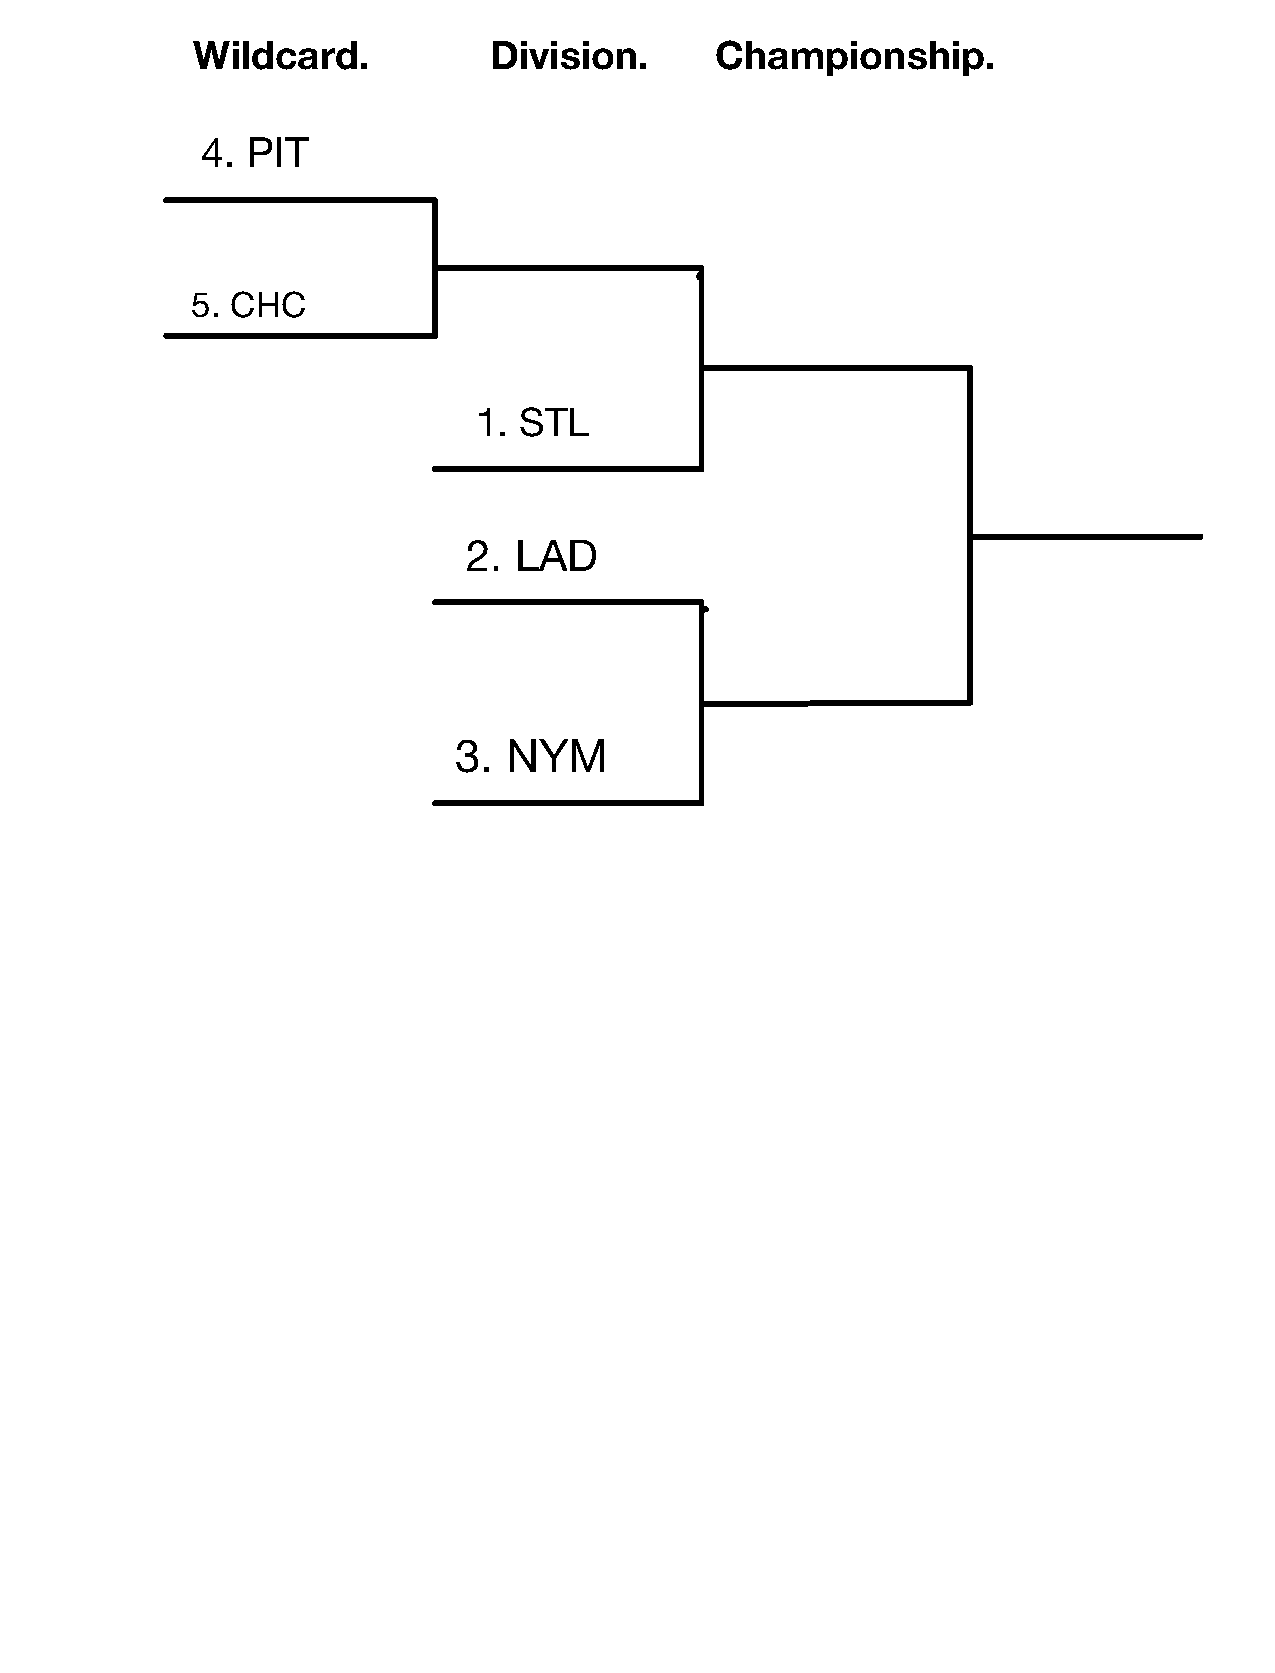
\includegraphics[height=13cm]{Bracket.pdf}
\end{center}


\subsection{Total Probability Rule}
This next rule gives another way to calculate the probability of an event. The idea is to ``break up'' the event $E$ into pieces.

\begin{center}
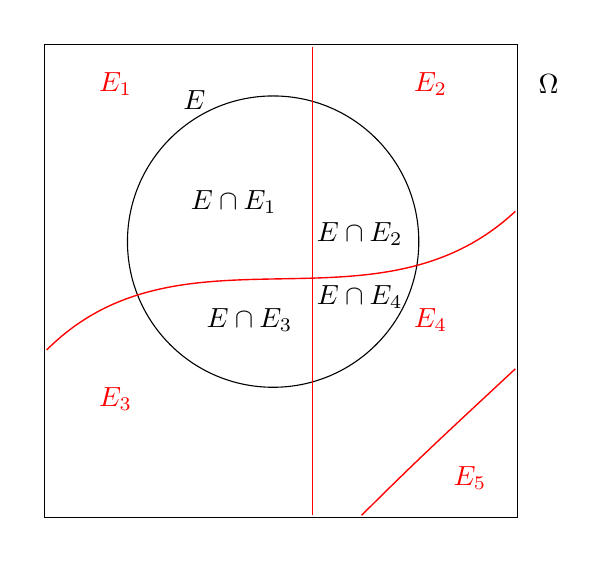
\begin{tikzpicture}
\draw [draw=black] (11.1,5.5) rectangle ++(6,6);
\filldraw [fill=white, fill opacity=0.2, draw=black] (14,9) circle (1.85);
\node at (13,10.8)  {$E$};
\node at (17.5,11) {$\Omega$};
\node at (14.5,11.6) (aa) {};
\node at (14.5,5.4) (a) {};
\node at (11.0,7.5) (bb) {};
\node at (17.2,9.5) (b) {};
\node at (15.0,5.4) (cc) {};
\node at (17.2,7.5) (c) {};
\draw (aa) edge[red,out=-90,in=90,-, line width=0.5pt] (a);
\draw (bb) edge[red,out=45,in=223,-, line width=0.5pt] (b);
\draw (cc) edge[red,out=45,in=223,-, line width=0.5pt] (c);
\node[red] at (12,11) {$E_1$};
\node[red] at (16,11) {$E_2$};
\node[red] at (12,7) {$E_3$};
\node[red] at (16,8) {$E_4$};
\node[red] at (16.5,6) {$E_5$};
\node at (13.5,9.5) {$E \cap E_1$};
\node at (13.7,8) {$E \cap E_3$};
\node at (15.1,9.1) {$E\cap E_2$};
\node at (15.1,8.3) {$E\cap E_4$};
\end{tikzpicture}
\end{center}


\begin{theorem} (Total Probability Rule)
Suppose $E_1,\ldots,E_n$ are disjoint events of positive probability such that $\bigcup_{i=1}^n E_i = \Omega$. Then for any $E\subseteq \Omega$, 
$$
\PP(E) = \sum_{i=1}^n \PP(E_i) \cdot \PP(E \vert E_i).
$$

\end{theorem}
\begin{proof}
Since $E\subseteq \Omega$, we have $E\cap \Omega = E$. Therefore
\begin{align*}
\PP(E) &= \PP(E \cap \Omega) \\
&= \PP\left( E \cap \left(\bigcup_{i=1}^n E_i \right)\right)
\end{align*}
We can the identity (this is called the distributive property -- the image above might help too)
$$
E \cap \left(\bigcup_{i=1}^n E_i \right) = \bigcup_{i=i}^n (E\cap E_i).
$$
So we have
$$
\PP(E) = \PP\left( \bigcup_{i=i}^n (E\cap E_i)\right).
$$
The events $E_i$ are disjoint (mutually exclusive), so this means that the events $E\cap E_i$ are too. By the additivity axiom,
$$
\PP(E) = \sum_{i=1}^n \PP(E\cap E_i).
$$
From the definition of conditional probability,
$$
\PP(E) = \sum_{i=1}^n \PP(E_i) \cdot \PP(E \vert E_i),
$$
as needed.






\end{proof}

A collection of disjoint events $\{E_i\}$ such that $\cup_i E_i = \Omega$ is sometimes called a \textit{partition} of $\Omega$. A simple partition is $E$ and its complement $E^c= \Omega - E$. Another example of a partition comes from random variables, which we will see below.

In the baseball example, we can ask for the probability that the Cardinals advance to the championship series. 

\subsection{Bayes' Rule}
Bayes' rule was developed by Thomas Bayes\footnote{Interesting note about Thomas Bayes: he was also a Presbyterian minister, and one of his published works was ``Divine Benevolence, or an Attempt to Prove That the Principal End of the Divine Providence and Government is the Happiness of His Creatures.''}, and is the foundation of Bayesian statistics.

\begin{theorem} (Bayes' rule)
Assume that $E\subseteq \Omega$ and $\PP(E)>0$. Then for any other event $E'$,
$$
\PP(E'\vert E) = \frac{\PP(E\vert E') \PP(E')}{\PP(E)}
$$
\end{theorem}
\begin{proof}
Plugging in the definition of conditional probability, we see that
\begin{align*}
 \frac{\PP(E\vert E') \PP(E')}{\PP(E)} &= \frac{\PP(E \cap E') \PP(E')}{ \PP(E') \PP(E)} \\
&=\frac{\PP(E \cap E')}{\PP(E)} \\
&= \PP(E'\vert E) 
\end{align*}
\end{proof}

Here is a very common example of Bayes' rule (called the ``false positive'' example). Suppose that there is a rare disease, which occurs in one out of every 1000 people. There is test for the disease which is 95\% accurate. If someone tests positive for the disease, what is the probability that they actually have the disease? (What's your gut instinct, if you didn't know math?)

The first step is to translate the problem from English to math (to be honest, the translating part is probably harder than the actual math part). When we have no information, we can say that 1/1000 of the population has the disease, so
$$
\PP(\text{disease})=0.001.
$$
If someone has the disease, the test will return a positive result 95\% of the time. This is a conditional probability statement:
$$
\PP(\text{positive} \vert \text{ disease }) =0.95.
$$
The question is asking for the value of the ``reversed'' conditioning:
$$
\PP( \text{disease} \vert \text{positive}) = ??
$$
Then we can apply Bayes' rule:
$$
\PP( \text{disease} \vert \text{positive}) = \frac{\PP(\text{positive} \vert \text{ disease }) \PP(\text{disease})}{ \PP(\text{positive}) }.
$$
We already know the value of the numerator. To find the denominator, we use the total probability rule to see that
$$
\PP( \text{disease} \vert \text{positive}) = \frac{\PP(\text{positive} \vert \text{ disease }) \PP(\text{disease})}{ \PP(\text{positive} \vert \text{healthy}) \PP(\text{healthy}) + \PP(\text{positive} \vert \text{disease}) \PP(\text{disease}) }.
$$
The exact value of the denominator is found by 
\begin{align*}
\PP(\text{positive}) &= \PP(\text{positive} \vert \text{healthy}) \PP(\text{healthy}) + \PP(\text{positive} \vert \text{disease}) \PP(\text{disease}) \\
&= (1-0.95)) (1-0.001) + (0.95) (0.001).
\end{align*}
So the answer is
$$
\frac{(0.95) (0.001)}{(1-0.95)) (1-0.001) + (0.95) (0.001)} \approx 0.0187.
$$
So the answer is actually less than two percent!


Some authors combine Bayes' rule and total probability rule, to write it as
$$
\PP(E'\vert E) = \frac{\PP(E\vert E') \PP(E') }{\PP(E\vert E') \PP(E')  + \PP(E\vert E'^c) \PP(E'^c)  }.
$$
(Recall that the complement of a set $A$ is everything not in $A$. Here that means $E^c = \Omega - E$).
Both are perfectly fine expressions of Bayes' rule (at this for this class). 

\subsection{Conditional Independence}
When we condition on an event, we have a new probability law on a new sample space. An interesting phenomenon is that this can also change the relationship between two events. We investigate this phenomenon when the relationship is independence.

\begin{definition}
Let $E\subseteq \Omega$ be an event of positive probability. We say that two other events $E_1,E_2\subseteq \Omega$ are \textit{conditionally independent given E} if
$$
\PP(E_1 \cap E_2 \vert E) = \PP(E_1\vert E) \cdot \PP(E_2 \vert E).
$$
\end{definition}

Conditional independence does not imply independence, and vice versa. We'll do an example (this is also an example to practice the total probability rule, and independence).

A jar contains two coins: a regular coin, and a two--headed coin. You pull a coin at random and then flip it twice. Define the three events
\begin{align*}
E_1 &= \{ \text{ first flip is heads}\}\\
E_2 &= \{ \text{ second flip is heads}\}\\
E_3 &= \{ \text{ you pulled the regular coin }\}.
\end{align*}
The events $E_1$ and $E_2$ are independent given $E_3$ (hopefully this is clear from the set up of the problem). Are $E_1$ and $E_2$ independent? What's your gut instinct? How would we find out?

Let's find the probabilities of $E_1,E_2,E_1 \cap E_2$ using the total probability rule.  First, note that $E_3$ and $E_3^c$ always form a partition. So
\begin{align*}
\PP(E_1) &= \PP(E_3)\PP(E_1 \vert E_3) + \PP(E_3^c)\PP(E_1 \vert E_3^c) \\
&= \frac{1}{2} \cdot \frac{1}{2} + \frac{1}{2} \cdot 1 \\
&= \frac{3}{4}.
\end{align*}
By an identical argument,
$$
\PP(E_2) = \frac{3}{4}.
$$
To find the probability $E_1\cap E_2$, we use the same partition:
\begin{align*}
\PP(E_1 \cap E_2) &= \PP(E_3)\PP(E_1 \cap E_2 \vert E_3) + \PP(E_3^c)\PP(E_1 \cap E_2 \vert E_3^c) \\
&=  \PP(E_3)\PP(E_1 \vert E_3) \PP( E_2 \vert E_3) + \PP(E_3^c)\PP(E_1 \vert E_3^c) \PP( E_2 \vert E_3^c) \text{  (by conditional independence) }\\
&= \frac{1}{2} \cdot \frac{1}{2} \cdot \frac{1}{2} + \frac{1}{2} \cdot 1 \cdot 1 \\
&= \frac{5}{8}.
\end{align*}
Since 
$$
\PP(E_1)\PP(E_2) = \frac{9}{16} \neq \PP(E_1 \cap E_2) = \frac{3}{4},
$$
they are not independent.


\newpage
\end{document}